% !TeX spellcheck = en_GB
\documentclass[10pt,letterpaper,oneside]{article}
\def\NoteAuthor{Chris Eliasmith}
\def\BasedOn{}
\usepackage{fontspec}
\usepackage{arev}
\usepackage[utf8]{inputenc}
\usepackage[T1]{fontenc}
\usepackage{amsmath}
\usepackage{amsfonts}
\usepackage{amssymb}
\usepackage{graphicx}
\usepackage{csquotes}
\usepackage{booktabs}
\usepackage{multicol}
\usepackage{enumerate}
\usepackage{microtype}
\usepackage[labelfont=bf,font={small}]{caption}
\usepackage{hyperref}
\usepackage{booktabs}
\usepackage{subcaption}
\usepackage{fancyhdr}
\usepackage[svgnames]{xcolor}
\usepackage{mdframed}
\usepackage{multicol}
\usepackage[para]{footmisc}
\usepackage{siunitx}
\usepackage{cleveref}
\usepackage{listings}
\usepackage{cprotect}


\lstset{ % General setup for the package
	language=Python,
	basicstyle=\small\ttfamily,
	tabsize=4,
	columns=fixed,
	showstringspaces=false,
	showtabs=false,
	keepspaces,
	commentstyle=\color{SeaGreen},
	keywordstyle=\bf\ttfamily\color{DarkBlue},
	stringstyle=\ttfamily\color{Crimson}
}

\newfontfamily\symbolfont{Symbola}
\usepackage[left=1in,right=1in,top=1in,bottom=1in,marginparwidth=0.3in]{geometry}

\usepackage[sorting=none]{biblatex}
\addbibresource{../bibliography.bib}

\ifx\NoteAuthor\undefined
  \def\NoteAuthor{Andreas Stöckel and Chris Eliasmith}
\fi

\ifx\BasedOn\undefined
  \def\BasedOn{Based on lecture notes by\\Chris Eliasmith and Terrence~C.~Stewart}
\fi

\author{\NoteAuthor\\[0.5cm]\BasedOn}
\newcommand{\baseCodeURL}{https://github.com/celiasmith/syde556-f24/blob/master/lectures}

\fancyhf{}
\fancyhead[L]{SYDE 556/750 Lecture Notes}
\fancyhead[R]{\NoteAuthor}
\fancyfoot[C]{\thepage}
\pagestyle{fancy}

\setlength{\parindent}{0em}
\setlength{\parskip}{0.5em}
\renewcommand{\baselinestretch}{1.25}

\renewcommand{\vec}[1]{{\mathbf{#1}}}
\newcommand{\mat}[1]{{\mathbf{#1}}}
\newcommand{\T}{\ensuremath{\mathrm{T}}}
\renewcommand{\epsilon}{\varepsilon}
\renewcommand{\phi}{\varphi}

\makeatletter
\newcommand{\superimpose}[2]{%
	{\ooalign{{#1}\hidewidth\cr{#2}\hidewidth\cr}}}
\makeatother
\newcommand{\SolidCircle}[2]{\superimpose{\color{#1}\symbolfont ⬤}{\textbf{\color{white}#2}}\hspace{1em}}
\newcommand{\OPlus}{\SolidCircle{DarkGreen}{\kern0.75pt+}}
\newcommand{\OMeh}{\SolidCircle{DarkOrange}{~}}
\newcommand{\OMinus}{\SolidCircle{DarkRed}{\kern2.25pt--}}

\newcommand{\YouTube}[2][Video]{\href{https://youtu.be/#2}{{\symbolfont 📺}~{#1}}%
%\footnote{\url{https://youtu.be/#2}}%
}

\newcommand{\CodeLink}[2][Code]{\href{\baseCodeURL/#2}{{\symbolfont ⌨}~\emph{#1}}}

\newcommand{\MakeTitle}[1]{
\maketitle
\begin{center}
	\includegraphics[width=0.5\textwidth]{../assets/uwlogo.pdf}\\[1cm]
	{#1}\
\end{center}

\vfill

\thispagestyle{empty}
\setcounter{page}{0}
\newpage

\pagenumbering{roman}
\setcounter{tocdepth}{2}
\tableofcontents
\newpage

\setcounter{page}{0}
\pagenumbering{arabic}}

\reversemarginpar


\newcommand{\ColorBox}[3]{%
	\marginpar{%
		\huge\raisebox{-3ex}{\symbolfont{#1}}%
	}%
	\begin{mdframed}[hidealllines=true,backgroundcolor=#2,innertopmargin=0.25cm,innerbottommargin=0.25cm]%
		{#3}
	\end{mdframed}}

\newcommand{\Note}[1]{\ColorBox{📌}{WhiteSmoke}{\textbf{Note:} #1}}
\newcommand{\Example}[1]{\ColorBox{💡}{WhiteSmoke}{\textbf{Example:} #1}}
\newcommand{\Aside}[1]{\ColorBox{🌟}{WhiteSmoke}{\emph{Aside:} #1}}
\newcommand{\Python}[1]{\ColorBox{🐍}{WhiteSmoke}{#1}}
\newcommand{\Notation}[1]{\ColorBox{\huge$\Sigma$}{WhiteSmoke}{\textbf{Notaton:} #1}}

\newcommand{\ConstructionSite}{\hrulefill {\symbolfont 🚧} UNDER CONSTRUCTION {\symbolfont 🚧} \hrulefill}

\newenvironment{ImportantEqn}[1]{\mdframed\raggedleft\emph{({#1})}\align}{\endalign\endmdframed}

\date{November 20, 2024}
\title{SYDE 556/750 \\ Simulating Neurobiological Systems \\ Lecture 14: Spatial Semantic Pointers}

\newcommand{\sinc}[1]{\operatorname{sinc}\left({#1}\right)}
\newcommand{\unbind}{\oslash}
\newcommand{\bind}{\circledast}
\newcommand{\analog}{\overset{C}{\approx}}
\newcommand{\domain}[1]{\mathcal{#1}}
\newcommand{\ssp}[1]{\mathrm{\uppercase{#1}}^{\lowercase{#1}/h}}
\newcommand{\sspi}[2]{\mathrm{\uppercase{#1}}^{\lowercase{#1}_{#2}/h}}

\begin{document}

\MakeTitle{\textbf{Accompanying Readings: Dumont \& Eliasmith, 2020. \href{http://compneuro.uwaterloo.ca/publications/dumont2020.html}{See here.}}}

\section{Introduction}

\Note{These notes are very under constructions, and mostly mathematical background. Much of the material is directly from Dumont and Eliasmith, 2020.}

We define circular convoluation exponentiation as: 
\begin{equation}
  B^k = \underbrace{B \circledast B \circledast \dots \circledast B. }_{\text{k times}}
\end{equation}

This can be written: 
\begin{equation}
  B^k = \mathcal{F}^{-1}\{\mathcal{F}\{B\}^k\}, \quad k \in \mathbb{R}
\end{equation}

where exponentiation in the fourier domain is regular exponentiation.  Where: 

\begin{align}
  \mathcal{F}\{ X\} &= r_{x} e^{i \theta_{x}} \\
  \textrm{So,}\\
  \mathcal{F}\{ X\}^x &= \left( r_{x} e^{i \theta_{x}} \right)^x \\
  &= r_{x}^x e^{i \theta_{x} x} 
\end{align}

Note that because we are working with exclusively unitary vectors, $r_x = 1$, and so the $\theta$ phases completely determine the SSP that is being used. If that were not the case, the magnitude would grow exponentially or collapse to zero with repeated binding.

We can write a 2D spatial representation as: 
\begin{equation}
  S(x,y) = X^x \circledast Y^y = \mathcal{F}^{-1}\{\mathcal{F}\{X\}^x\odot\mathcal{F} \{Y\}^y\},
\end{equation}

where $\odot$ is the Hadamard (element-wise) product. In the frequency domain: 
\begin{align}
  S(x, y) &= (X^{x} \circledast Y^{y}) \\
   &= \mathcal{F}^{-1}( \mathcal{F}\{ X\}^{x} \odot \mathcal{F}\{ Y\}^{y} ) \\
   &=  \mathcal{F}^{-1}(r_{x}^x e^{ i \theta_{x} x} r_{y}^y  e^{i \theta_{y} y })\\
   &=  \mathcal{F}^{-1}(r_{x}^x r_{y}^y e^{ i(\theta_{x} x + \theta_{y} y )})
   &=  \mathcal{F}^{-1}(e^{ i(\theta_{x} x + \theta_{y} y )})
\end{align}

where we have left off the vector indexes for clarity, but note that the $\theta$ for each dimension can be different.

\section{Grid cells}
In the above, and initial characterization of SSPs, we do not enforce any particular structure on the SSP axis vectors. However, we can choose the axis vectors to have a specific structure to get grid-like representations. To begin, let us consider an argument for why grid cells are useful for representing space.

Suppose ideal place cells are Gaussian bumps, and that they evenly cover a space to be represented. We would like to find the hidden layer activations $G \in \mathbb{R}^{n_x \times n_g}$ (where $n_g$ is the number of hidden neurons and $n_g < n_p$, and $n_p$ is the number of place cells) and the matrix of read-out weights $W \in \mathbb{R}^{n_g \times n_p}$ that minimize the reconstruction error of the place cell responses.
\begin{align}
\min_{G,W} || P - \hat{P} ||_{F}^2, \\ \hat{P} = GW
\end{align}
The optimal $W$ for a fixed $G$ is given by
\begin{equation} \label{eqn:optimReadOutWeight}
W^* = (G^T G)^{-1} G^T P.
\end{equation}
This $W$ should be thought of as the connection weights between the final two layers of some deep neural network. The input to the full network would be low level sensory information and the output would be the place cell activity, $P$. The hidden layer with activations $G$ is the last layer before the place cells, and, since $n_g < n_p$, it creates an information bottleneck. We are interested in finding the optimal $G$ - a compressed representation of spatial position that is optimal for reconstructing $P$ in a single layer.

As stated in \cite{sorscher2019unified}, if the number of place cells is large and their receptive fields uniformly cover space (and space has periodic boundary conditions) then $PP^T$ will approximately be a circulant matrix and its eigenvectors will be Fourier modes.

Thus, the optimal responses of hidden neurons will be linear combinations of plane waves. This will produce hidden neurons with grid-like spatial responses. Adding a non-negativity constraint to this optimization problem will result in the activity of an individual hidden neuron being proportional to a sum of three plane waves whose wave vectors are 120$^o$ degrees apart. Specifically, a column of $G$ will have entries,
\begin{align}
     \sum_{j=1}^{3} & e^{i \mathbf{k}_j \cdot \mathbf{x}_n } + e^{-i \mathbf{k}_j \cdot \mathbf{x}_n  } \label{eqn:planewavesum} \\
    \text{where } \quad & |\mathbf{k}_j| = |\mathbf{k}_i| \quad \forall i,j \\
    & \quad \sum_{j=1}^{3} \mathbf{k}_j = 0
\end{align}

The interference pattern of these waves will have a hexagonal grid pattern, like grid cells. Note that this is also real as the imaginary parts cancel. The first equation will show the interference patterns of the choice of $\mathbf{k}$ vectors -- i.e. be the grid cells in $G$.

It might be helpful to recall Euler's formula: 
\begin{align}
   e^{i x} = \cos(x) + i \sin(x)
\end{align}
to show that equation \ref{eqn:planewavesum} is:
\begin{align}
  \sum_{j=1}^{3} & e^{i \mathbf{k}_j \cdot \mathbf{x}_n } + e^{-i \mathbf{k}_j \cdot \mathbf{x}_n } \\
  =&  \sum_{j=1}^{3} \cos(\mathbf{k}_j \cdot \mathbf{x}_n) + i \sin(\mathbf{k}_j \cdot \mathbf{x}_n) + \cos(\mathbf{k}_j \cdot \mathbf{x}_n) - i \sin(\mathbf{k}_j \cdot \mathbf{x}_n) \\
  =& 2 \sum_{j=1}^{3} \cos(\mathbf{k}_j \cdot \mathbf{x}_n)
\end{align}

which defines the interference pattern we see as grid-like for the appropriate choice of $\mathbf{k}$. Changing the orientation of the $\mathbf{k}$ will rotate the grid, and changing the length of the $\mathbf{k}$ will change the spatial frequency (i.e., spacing) of the grid.

Returning to SSPs, we might ask if there is a way to choose the axis vectors, $X$ and $Y$ such that the resulting spatial representation is grid-like. That is, can we impose specific structure on the axis vectors to get grid cells? First, note that we can write multi-dimensional SSPs as:
\begin{align}
S(\vec{x})=\mathcal{F}^{-1}\left\{\mathrm{e}^{\mathrm{i}(A \vec{x})}\right\}
\end{align}
where $A$ is a matrix whose columns are the axis vectors, and $\vec{x}$ is the 2D space we are representing. Until now, we just pick random axis-vectors, which would be random phases in the two columns of $A$, chosen from an even distribution around the unit circle. We call these RandSSPs. Instead, we can pick the columns and rows carefully, such that the resulting spatial representation is grid-like. We call these HexSSPs. Specifically, if we pick the rows of A to be the vertices of an equilateral triangle (in 2-dimensions, or more generally, the $m$-dimensional simplex), i.e. the $\vec{k}$ vectors above, we will get grid-like representations (see Figure \ref{fig:SSP_kernels.pdf}A). 

We can then rotate and scale those base $\vec{k}$ vectors to get different grid spacing and sizes. As shown in Figure \ref{fig:SSP_kernels.pdf}A, the number of rotated vectors will determine the spacing of rings in the representation, and the number of scaled vectors will determine the smoothness of the representation. As shown in Figure \ref{fig:SSP_kernels.pdf}B, the HexSSP is much better than the RandSSP for estimating a smooth point function.

\begin{figure}
  \centering
  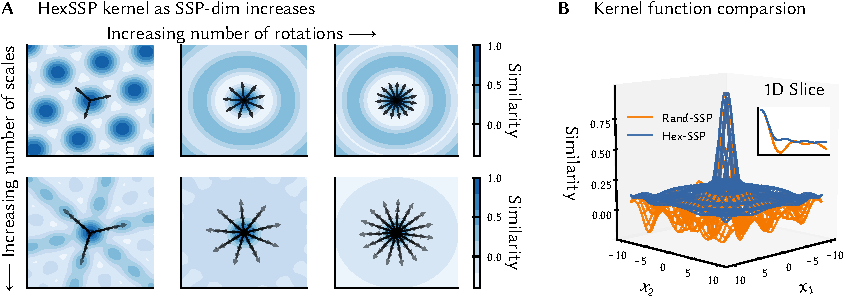
\includegraphics[width=\linewidth]{media/SSP_kernels.pdf}
  \caption{HexSSPs. \textbf{(A)} Interference patterns induced by HexSSPs representing points in a 2D space as a heat map. The initial 3-vector structure (top left) produces hexagonal interference patterns like those found in grid cell neurons.  Adding rotated versions (top right) produces a surface with a central peak surrounded by rings.  Increasing the number of rotated vectors (bottom left) results in a starburst pattern. Adding many rotated and scaled vectors (bottom right) reduces the magnitude of the surrounding rings and increases smoothness and robustness to noise. \textbf{(B)} RandSSPs result in a sinc kernel function, while HexSSPs produce a sum of sinc functions, making local maxima and minima more shallow. Figure from \cite{furlong2024bo}.}
  \label{fig:SSP_kernels.pdf}
\end{figure}


\section{Mathematical properties}

The most critical mathematical property that SSPs have is that they preserve Euclidean relations in a much higher dimensional space. That is, 
\begin{align}
   S(x_1,y_1) \circledast S(x_2,y_2) 
   &= S(x_1 + x_2,y_1 + y_2) \\
   &= X^{x_1 + x_2} \circledast Y^{y_1 + y_2}
\end{align}

So it's easy to shift a current spatial representation around without decoding the representation. We can use this to implement basic differential equations \cite{voelker2021a}:
\begin{equation} \label{eq:discrete-binding}
  S_{t + \Delta t} = \left ( X^{\Delta x_t} \circledast Y^{\Delta y_t} \right ) \circledast S_{t}  \text{,}
\end{equation}

where $\Delta x_t$ and $\Delta y_t$ are derived from differential equations that relate $x$ and $y$ to $t$. Assuming $ S_{t}=X^{x_t} \circledast Y^{y_t}$, then the algebraic properties of SSPs ensure that: 
\begin{align}
  & X^{x_t} \circledast Y^{y_t} \circledast X^{\Delta x_t} \circledast Y^{\Delta y_t} \\
  &= X^{x_t + \Delta x_t} \circledast Y^{y_t + \Delta y_t} 
\end{align}

It's also possible to write a similar equation without discretizing time. The result of doing so gives: 
\begin{equation} \label{eq:continuous-binding}
  \frac{d S }{dt} = \left( \frac{dx}{dt} \ln X + \frac{dy}{dt} \ln Y \right) \circledast S \text{.}
 \end{equation}

Of relevance to using SSPs as probability representations, it's important to note that as the dimensionality becomes sufficiently high, the expected similiarity approaches:
\begin{equation}
X^{x_1} \cdot X^{x_2} = \sinc{x_2 - x_1}
\end{equation}
for SSPs~\cite{voelker2020short}.




\section{Probabilities}

This section is based on \cite{furlong2022fractional}. Assume a fixed dataset, $\mathcal{D} = \{x_{1},\ldots,x_{n}\mid x_{i} \in \mathbb{R}^{m}\}$ of $n$ samples of $m$-dimensional data. 

We use a length scale parameter, $h$, so when we write $\ssp{x}$ we mean $\mathcal{F}^{-1}\left\{\mathrm{e}^{\mathrm{i}\theta_{X}x/h}\right\}$, for $x \in \mathbb{R}^{m}$. This parameter essentially normalizes the SSPs over the appropriate domain given the number of samples. You can find the optimal length scale for the estimator we discuss below, but it is beyond our scope.

We define our estimator as: 
\begin{align}
  \hat{f}(x\mid \mathcal{D}) = \ssp{x}\cdot \frac{1}{nh}\sum_{x_{i} \in \mathcal{D}} \sspi{x}{i}
\end{align} 

For any domain space $x \in X \subseteq \mathbb{R}^{m}$, we will denote the normalized sum as:
\begin{align}
M_{X,n} = \frac{1}{nh}\sum_{x_{i} \in \mathcal{D}}\sspi{x}{i}
\end{align}

Recall that we know that the dot product between SSPs induces a sinc function.  This is a 'quasi'-kernel because it takes on negative values. So our estimator is not a Kernel Density Estimator (KDE; a common kind of density estimatory), but a special-case Fourier Integral Estimator (FIE). FIEs can be converted to probability density estimators with a correction.

The particular correction for the FIE is:
\begin{align}
  f_{X}(x) \approx \max\left\{0,\hat{f}_\mathrm{FIE}\left(x \mid \mathcal{D}\right)-\xi\right\}
\end{align}
$\xi\in \mathbb{R}$ is selected so $\int_{-\infty}^{\infty}\max\left\{0,\hat{f}_\mathrm{FIE}\left(x \mid \mathcal{D}\right)-\xi\right\}dx = 1$. The particular correction for our estimator is: 
\begin{align}
  f_{X}(x) \approx \max\left\{0,\ssp{x}\cdot M_{X,n} - \xi\right\}
\end{align}

Which looks like a ReLU with a bias of $\xi$. Interestingly, we can think of either the $X$ or $M$ as connection weights (and the other as activities). Which we choose will lead to different implementation architectures.

Interestingly, unbinding this kind of representation can be thought of as computing a conditional distribution.  Briefly, 
\begin{align}
  g(X) = f(X,Y=y) \analog \ssp{x}\bind Y^{0}\cdot \sum_{x_i,y_i \in \mathcal{D}} \sspi{x}{i}\bind Y^{\frac{y_{i}-y}{h}}
\end{align}

Recognizing that 
\begin{align}
  f(X\mid Y=y) = \frac{1}{\eta}f(X,Y=y)
\end{align}
means unbinding can be seen as a non-normalized conditioned distribution. There are various ways we might compute the normalization constant $\eta \approx \int_{-\infty}^{\infty}\|\ssp{X}\cdot M_{X\mid Y,n}\|^{2} dx$.

We can similarly perform marginalization with SSP operations:
\begin{align}
  f_{X}(x) &= \int_{\domain{Y}}f_{XY}(x,y)dy \\
  &\analog \int_{\domain{Y}}\ssp{X}\bind\ssp{Y} \cdot \left(\sum_{(x_{i},y_{i}) \in \mathcal{D}}\sspi{X}{i}\bind\sspi{Y}{i}\right)dy \\
  &\analog \left(\ssp{X}\bind\int_{\domain{Y}}\ssp{Y}dy\right) \cdot \left(\sum_{(x_{i},y_{i}) \in \mathcal{D}}\sspi{X}{i}\bind\sspi{Y}{i}\right)
\end{align}

The integral over $y$ is a vector we can approximate by sampling $Y$. If we let:
\begin{align}
  \Phi_{Y} = \int_{\domain{Y}}\ssp{Y}dy\text{,}
\end{align}
then
\begin{align}
  f_{X}(x) \analog \left(\ssp{X}\bind\Phi_{Y}\right) \cdot M_{XY,n}.
\end{align}

Noting that circular convolution can be written as a matrix-vector product between one argument and the circulant matrix, $\mathrm{Circ}(\cdot)$, of the other argument, we can make the following simplification:
\begin{align}
  \left(\ssp{X}\bind\Phi_{Y}\right) \cdot M_{XY,n} &= \left(\mathrm{Circ}(\Phi_{Y})\ssp{X}\right)^{T} M_{XY,n}\\
  &= \ssp{X}\cdot\left(\mathrm{Circ}(\Phi_{Y})^{T} M_{XY,n}\right)
\end{align}

So the circulant is a linear map that marginalizes $M$.

See the original paper for examples pertaining to entropy estimation and mutual information calculation.  The latter is what is used to solve the search problem shown in the slides.

\printbibliography

\end{document}

